\documentclass[]{report}
\usepackage{graphicx}

% Title Page
\title{A Report into the Relationship between Tax, GDP and Regulatory Environment}
\author{Your name goes here}


\begin{document}
\maketitle

\begin{abstract}
A Report compiled for the Alliance of Wealthy People who Dislike Tax, investigating the relationship between rates of taxation (measured as a percentage of GDP), regulatory environment (measured through the World Bank's Ease of Doing Business), and GDP per capita (measured in current US dollars). Data are for European and Central Asian countries for the year 2019.
\end{abstract}

\section{Findings}
A multivariate regression of the variables resulted in the following findings:

% paste your stargazer code here
\begin{table}[!htbp] \centering 
	\caption{} 
	\label{} 
	\begin{tabular}{@{\extracolsep{5pt}}lc} 
		\\[-1.8ex]\hline 
		\hline \\[-1.8ex] 
		& \multicolumn{1}{c}{\textit{Dependent variable:}} \\ 
		\cline{2-2} 
		\\[-1.8ex] & GDP per capita (US dollar) \\ 
		\hline \\[-1.8ex] 
		Tax revenue (\% of GDP) & 1,458.236$^{*}$ \\ 
		& (738.971) \\ 
		& \\ 
		Ease of doing business rank & $-$222.973 \\ 
		& (162.657) \\ 
		& \\ 
		Constant & 9,256.393 \\ 
		& (17,201.770) \\ 
		& \\ 
		\hline \\[-1.8ex] 
		Observations & 46 \\ 
		R$^{2}$ & 0.133 \\ 
		Adjusted R$^{2}$ & 0.092 \\ 
		Residual Std. Error & 24,895.280 (df = 43) \\ 
		F Statistic & 3.290$^{**}$ (df = 2; 43) \\ 
		\hline 
		\hline \\[-1.8ex] 
		\textit{Note:}  & \multicolumn{1}{r}{$^{*}$p$<$0.1; $^{**}$p$<$0.05; $^{***}$p$<$0.01} \\ 
	\end{tabular} 
\end{table} 

The relationship can be visualised in a scatter plot.
%this will only work if you saved your plot as Rplot.pdf!
\begin{figure}[b!]\centering
	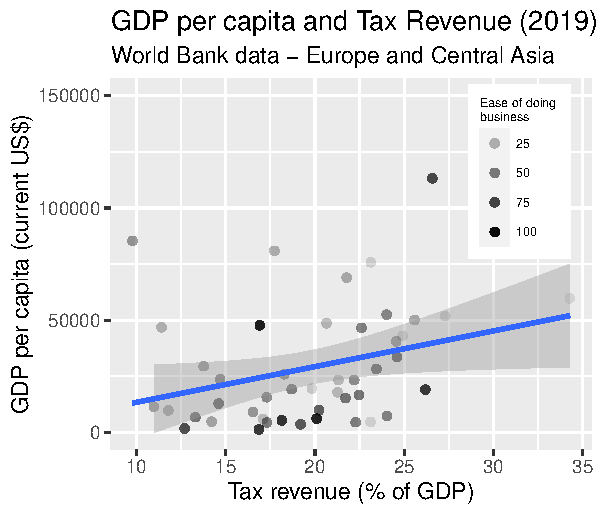
\includegraphics[width=.7\textwidth]{Rplot.pdf}\\
\end{figure}

\end{document}          
